\newpage
\setcounter{page}{1}
\justifying
\noindent

\section{Introduction}
\subsection{Formula Student}
Formula Student United Kingdom (FSUK) is an annual motor-sport engineering competition held by the Institute of Mechanical Engineers (IMechE). Every July since 2007, hundreds of universities from around the world have gathered at the Silverstone Circuit for the final competition. Every team's objective is to design and build a single-seat race car, which will be judged on several engineering and business aspects. The competition mainly consists of two events: static and dynamic. The static event judges the Engineering  Design,  Cost, and  Sustainability  Analysis; Business Presentation; and Technical Inspection, and the dynamic event evaluates Skid Pad; Sprint; Acceleration; Endurance; and Fuel.

\begin{figure}[!ht]
\begin{center}
%    
  \begin{subfigure}[b]{0.45\textwidth}
    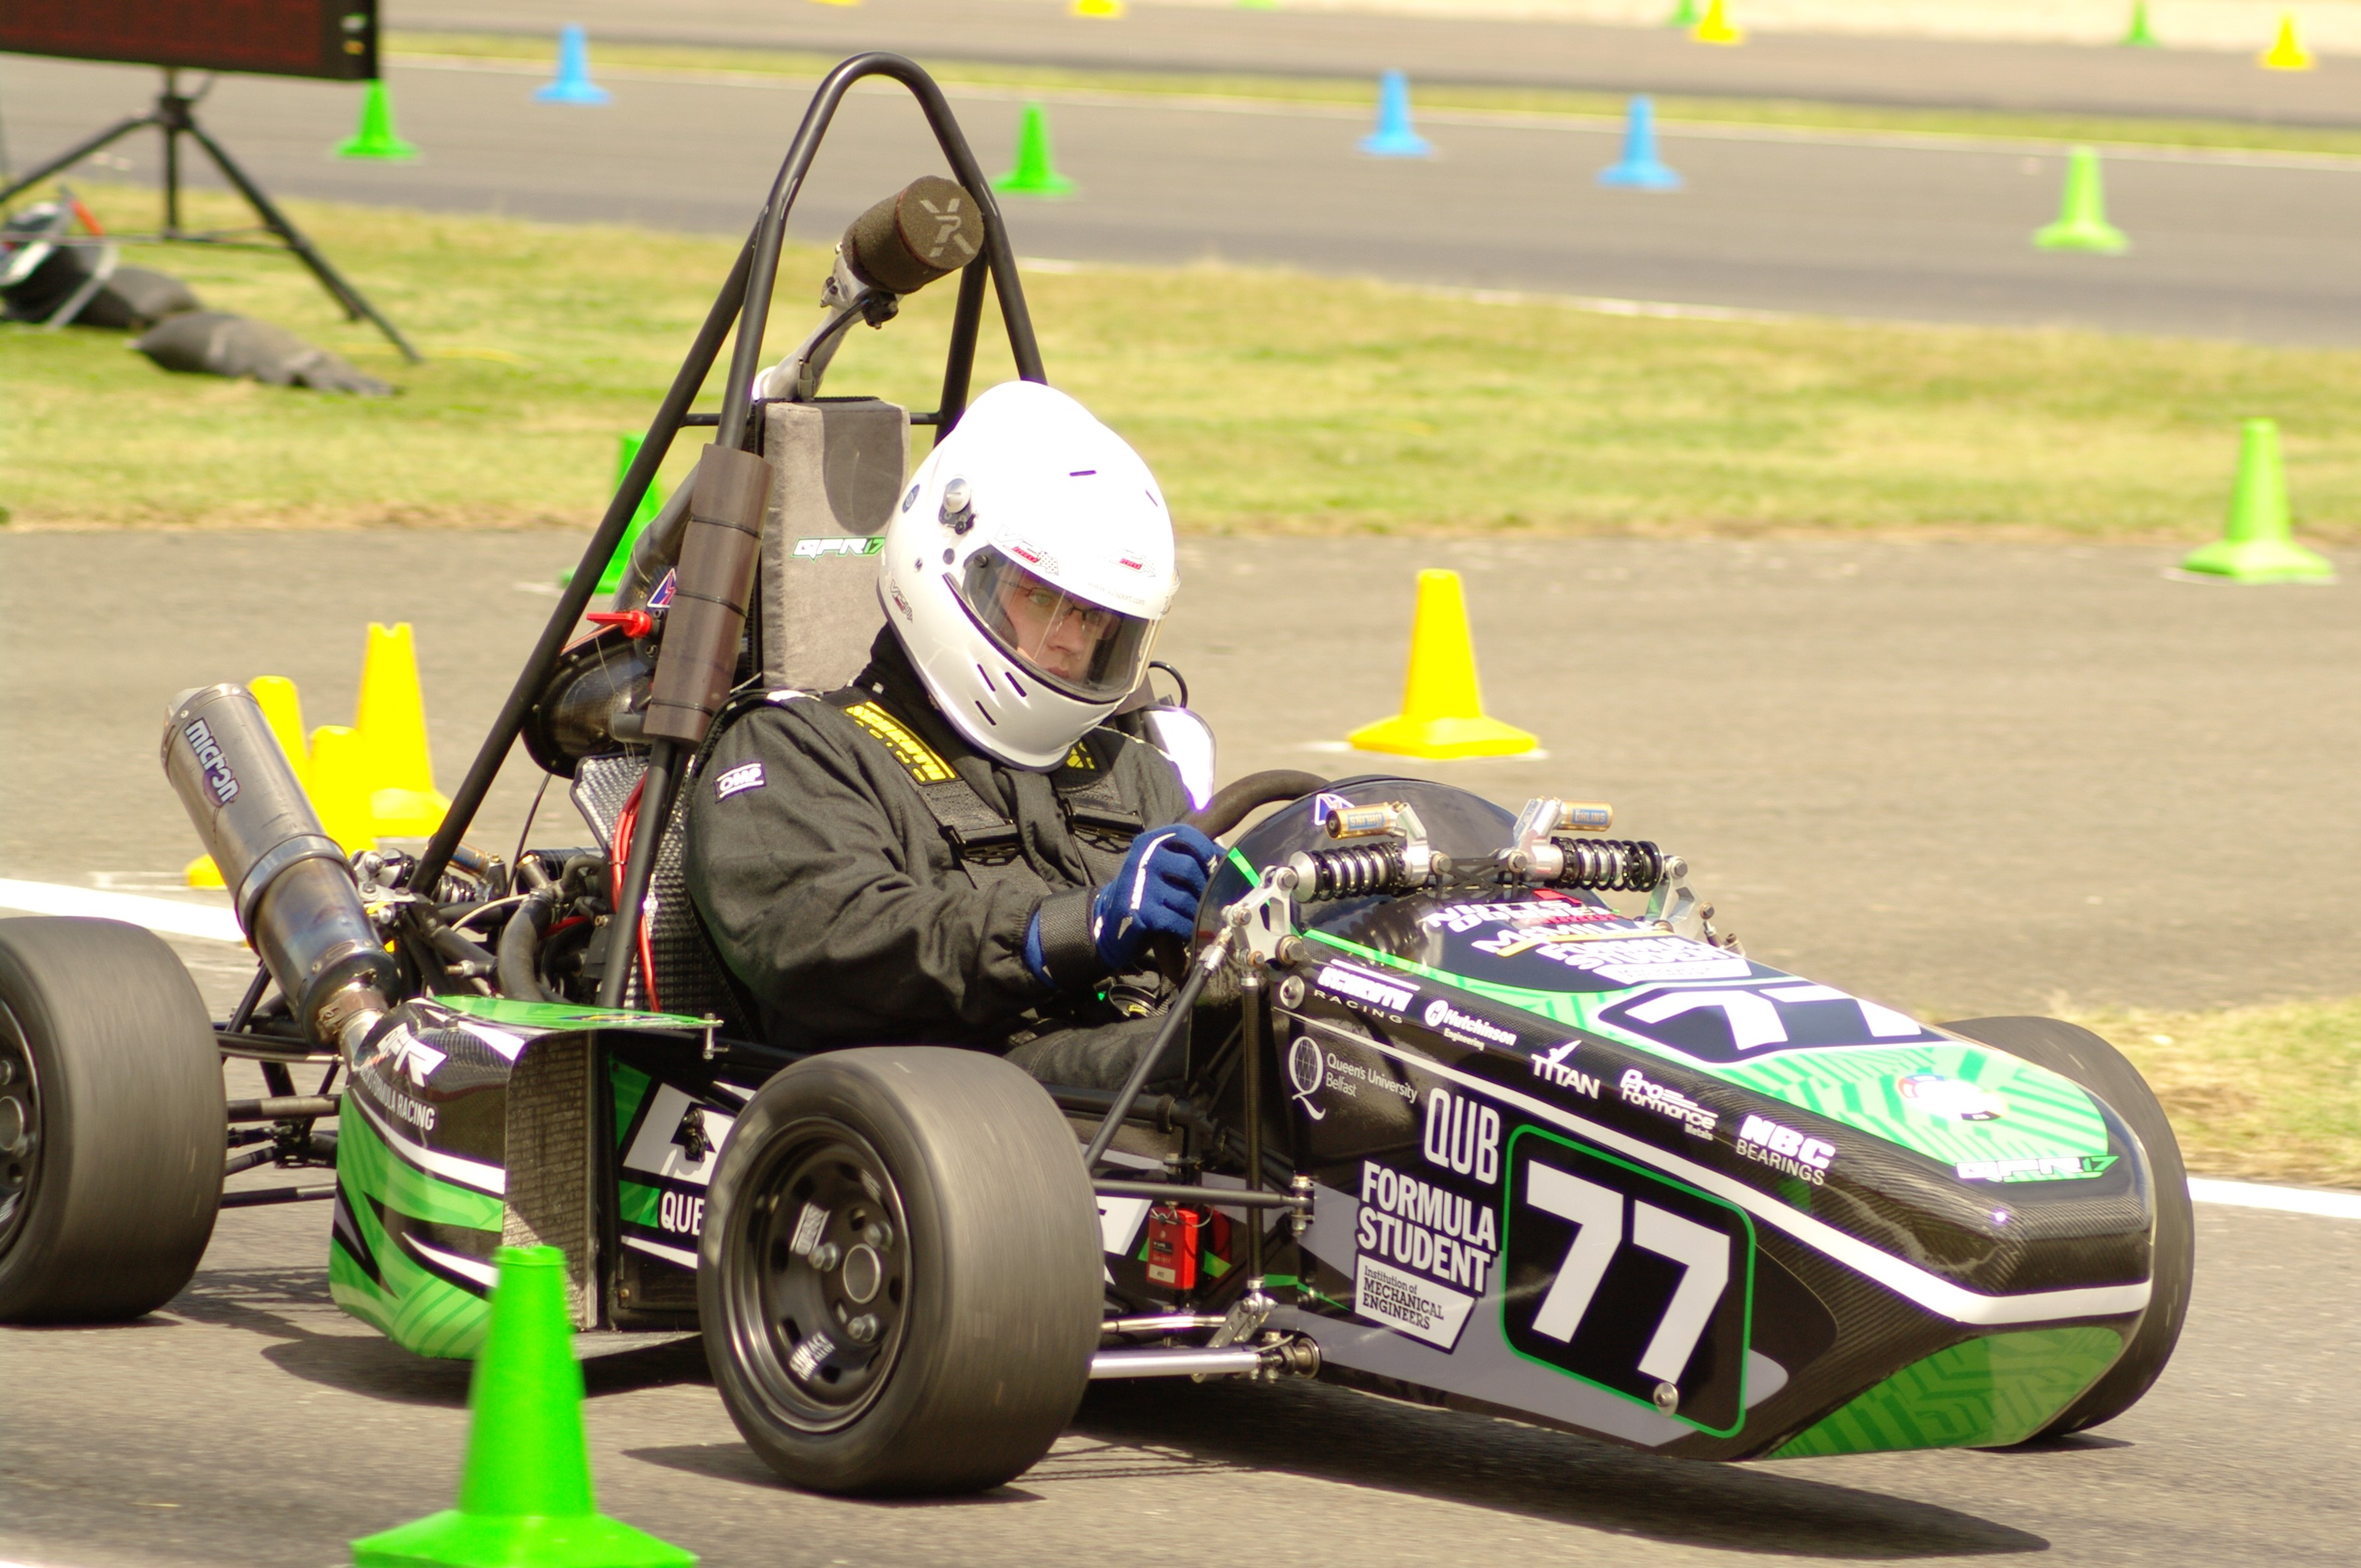
\includegraphics[height=4.5cm]{Figures/QFR17PHOTO.JPG}
  \end{subfigure}
  %
  \begin{subfigure}[b]{0.45\textwidth}
    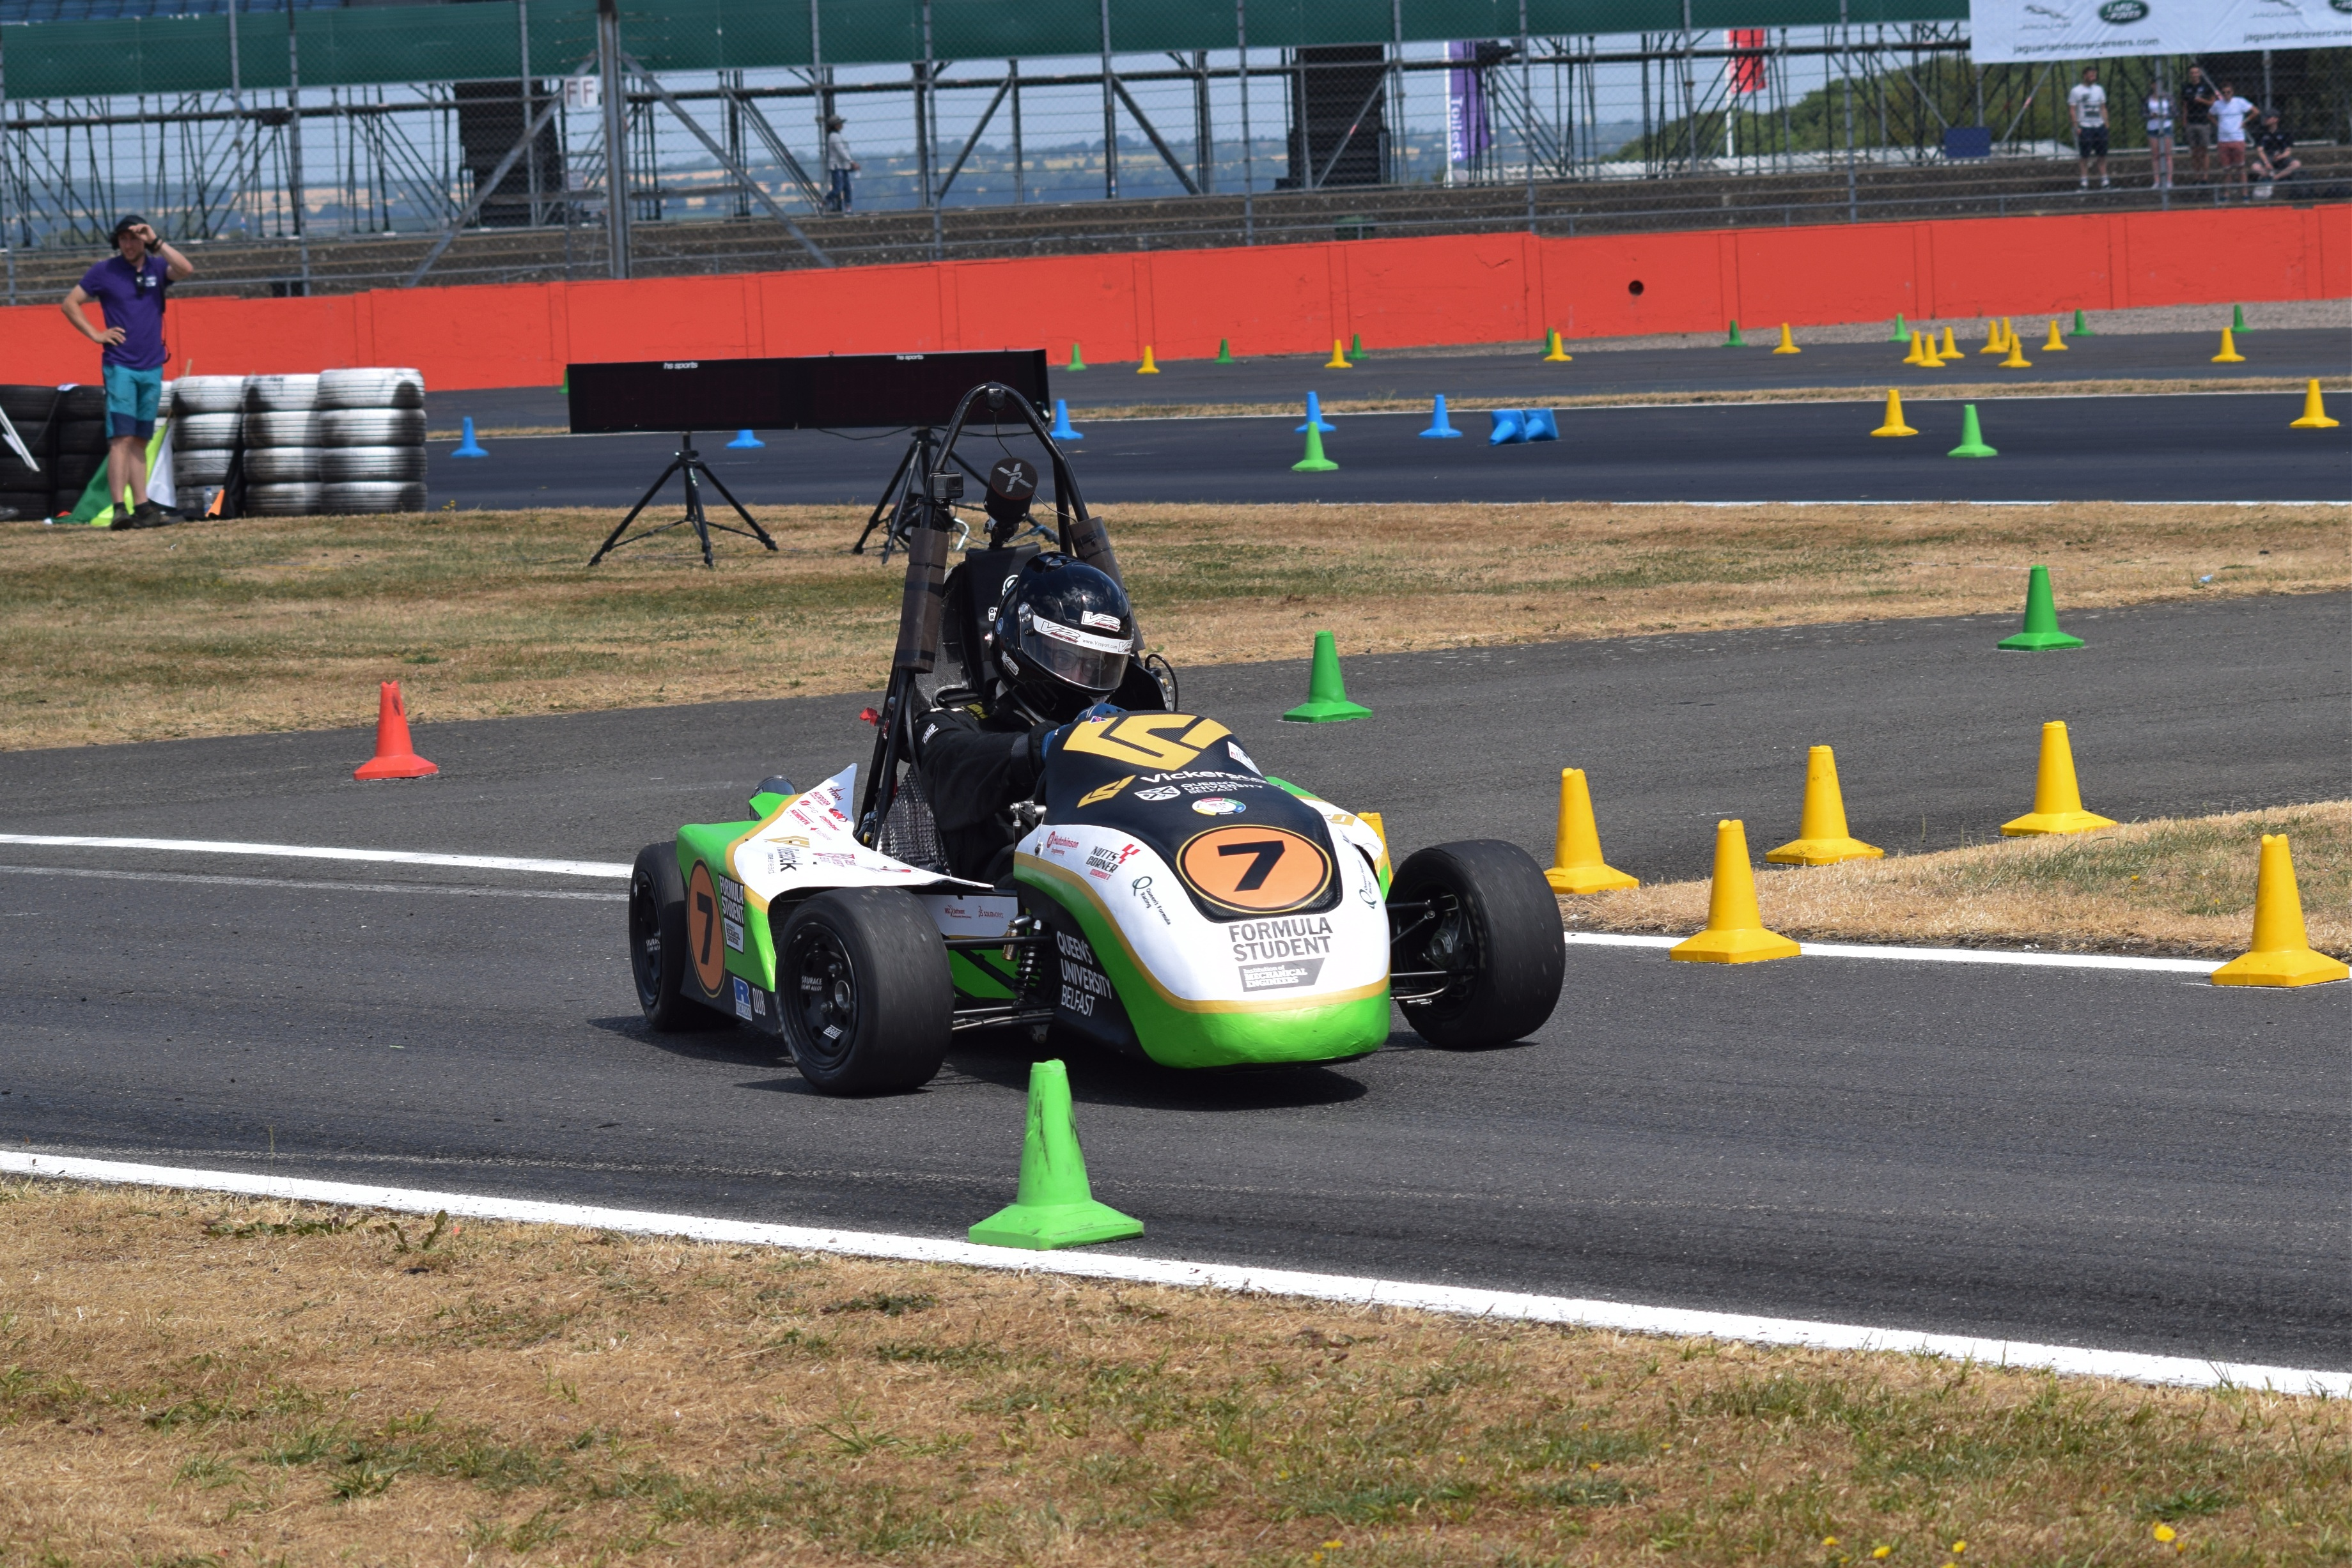
\includegraphics[height=4.5cm]{Figures/QFR18PHOTO.jpg}
  \end{subfigure}
%  
  \caption{Queen's Formula Racing Car 2017 (left) and 2018 (right) On the Dynamics Event}
    \label{fig:1}
\end{center}
\end{figure}

\noindent Queen's Formula Student first initiated consideration of aerodynamic aspects on the QFR car in 2017, which focused on the aerodynamic analysis framework \cite{Corr2017MechanicalAuthor}. In 2018, the first design of an aerodynamic undertray for the QFR race car was generated \cite{McKeown2018DesignCar}. This paper is intended to build on the analyses from previous projects, and to improve the undertray performance by investigating broader and deeper variables that could plausibly enhance the performance of the car as a whole. 

\subsection{The Significance of Aerodynamics in Formula Industry}
Aerodynamics has become a crucial aspect of high-speed car performance. The race-car industry has led technology innovation by indicating the need for constant improvement \cite{Zhang2006GroundCars}. Engineers have been striving to sculpt the shape of the cars to manipulate and take advantage of the flow round the body. The role of aerodynamics in improving race-car performance rose to prominence in 1968, when an inverted airfoil was first introduced to a Formula One car, and the research in this area has been growing exponentially ever since.

%put inverted aerofoil race car photo here

\noindent Downforce (negative lift) is an important aerodynamic effect, and is key in improving overall car performance. Downforce is produced by the flow of air around the body. This is usually achieved on a high-speed ground vehicle by introducing aerodynamic devices such as wings and undertrays, which modify the airflow to suit the engineering needs \cite{Wright1982TheCars}. In the race-car industry, the primary aim is to maximise the downforce while maintaining the lowest possible drag \cite{Zhang2006GroundCars}, but achieving consistent performance at diverse speeds and maximising acceleration is also essential. The magnitude of the downforce significantly affects braking, acceleration, and cornering --- and hence the cornering speed. Despite the restrictive aerodynamics rules in the competition, optimising the downforce could improve the acceleration, increasing the chance to overtake the opponent on a corner. Higher downforce can also allow the top speed to be reached more quickly, reducing corner entry and exit time. 

\noindent However, the ground-effect aerodynamics that applies to an open-wheeled car is still an experimental science \cite{Zhang2006GroundCars}. This is due to the complex flow physics that involves the interaction of a turbulent wake, the ground boundary layer, dynamic suspension motion, and many more factors, in which accurate analytical capability (both experimental \& computational) is not yet sufficiently developed.

\noindent Nevertheless, computational fluid dynamics (CFD) has improved tremendously within the industry over the years and has produced accurate results of forces, flow pattern, etc., in some particular car geometries. However, one research paper \cite{Zhang2006GroundCars} stated that race car diffuser is one of the most complex parts, the physics of which is hardly understood. Therefore, specific variables in generating an undertray geometry is required, with careful consideration of the assumptions on which the analysis is based.

\noindent This project will utilise CFD to understand the trends in behaviour of an aerodynamic undertray in both two and three dimensions, with several nozzle and diffuser variables such as angle, length, and width. These results will then be used to design a geometry for the final aerodynamic undertray of QFR 2021.

